 \documentclass[a4paper, 10pt, final]{article}

\usepackage{a4wide}

\usepackage{charter}
\usepackage{verbatim}
\usepackage{amsfonts}
\usepackage{amsmath}
\usepackage{amsthm}
\usepackage{amssymb}
%\usepackage[integrals]{wasysym}
%\usepackage{mathrsfs}
%\usepackage[mathcal]{euscript}
\usepackage{listings}
\usepackage{graphicx}
\usepackage{multirow}
\usepackage{multicol}
\usepackage{hyperref}
\usepackage{float}
\usepackage[small,bf]{caption}
\usepackage{synttree}
%\usepackage{pst-node}
%\usepackage{xypic}
\usepackage[table]{xcolor}
\usepackage{subfig}
%\usepackage{ulem} %use \normalem after begin document
\usepackage[authoryear]{natbib}

% Settings
\parindent=5pt
\parskip=8pt plus 2pt minus 4pt
\lstset{language=Matlab, basicstyle=\scriptsize,
    showstringspaces=false, numbers=left, stepnumber=1, numberstyle=\tiny, frame=tb}


\title{Statistical Methods for Machine Learning \\ Mandatory Project 2}
\author{Kasper Steenstrup\\Michael Andersen\\Esben Skaarup}
\date{\today}

\hypersetup{
colorlinks,%
citecolor=black,%
filecolor=black,%
linkcolor=black,%
urlcolor=black,%
bookmarksopen=false,
pdftitle={Statistical Methods for Machine Learning - Mandatory Project 2},
pdfauthor={Kasper Steenstrup, Michael Andersen \& Esben Skaarup}
}

\begin{document}
\maketitle

\subsection*{Question 2.1}

We calculate the RMS error for the two models, this is displayed in
table \ref{tab:q21} along with the min and max averaged over 50
iterations. In the first model the RMS error is lower than the other,
the first model min and max is also closer. Based on this fact, we see
that the first model is better, this was to be expected as the first
model is based on four features from the dataset and the second model
is based on one features from the dataset.

\begin{table}[!htbp]
  \centering
  \begin{tabular}{| l | l | l | l |}
    \hline
    {}		& RMS		& Max		& Min \\
    \hline
    Train1	& 4.4071	& 4.5634	& 4.2075 \\
    \hline
    Test1	& 4.5723	& 5.3269	& 3.9773 \\
    \hline
    Train2	& 4.8466	& 5.0046	& 4.5746 \\
    \hline
    Test2	& 4.9268	& 6.0025	& 4.2679 \\
    \hline
  \end{tabular}
  \caption{Shows the Root mean square, along with maximum and minimum.}
  \label{tab:q21}
\end{table}

\newpage


\subsection*{Question 2.2}
In figure \ref{fig:q22} the four RMS errors for $\alpha$ in the
interval from 1--200. As the figure indicates the test data, have the
lowest error, and the firste model have the best results, due to the
fact that it uses more features from the dataset to train the
model. The best value of $\alpha$ is one, since the error get bigger
the larger $\alpha$.

\begin{figure}[!htbp]
  \centering
  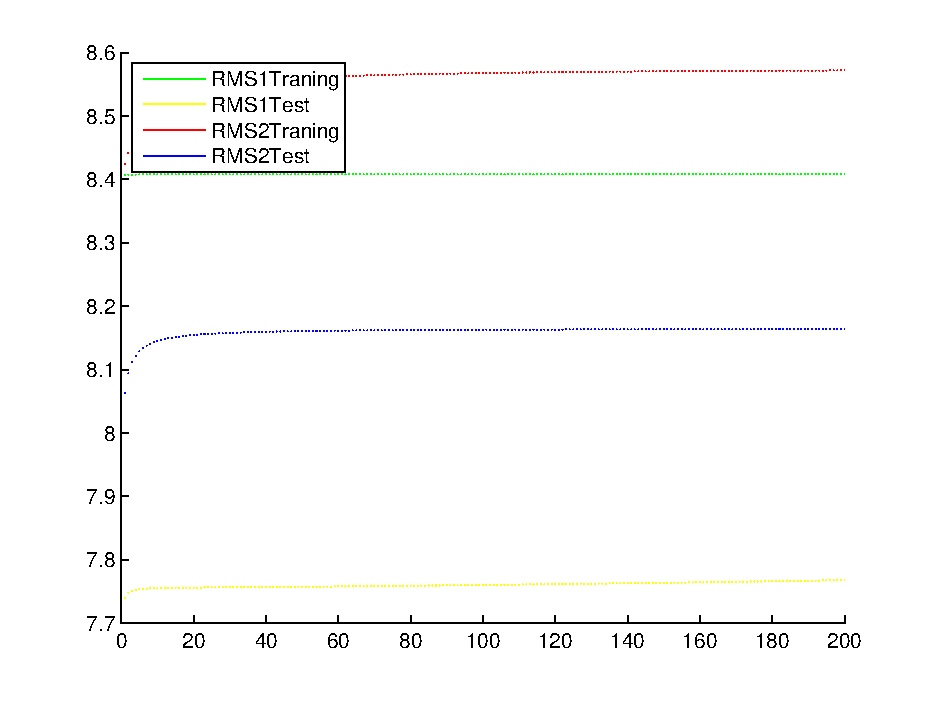
\includegraphics[width=0.75\textwidth]{./images/Q2.pdf}
  \caption{RMS for the two training models and test models}
  \label{fig:q22}
\end{figure}



In figure \ref{fig:q23a}, the original prediction trend,
$p(\mathbf{x}|\mathcal{C}_k)$ is displayed. In figure \ref{fig:q23b}
the prediction trend and Bayes classification is displayed. It can be
seen, that the two figures are very much alike, but some small
differences have happened.

\begin{figure}[!htbp]
  \centering
  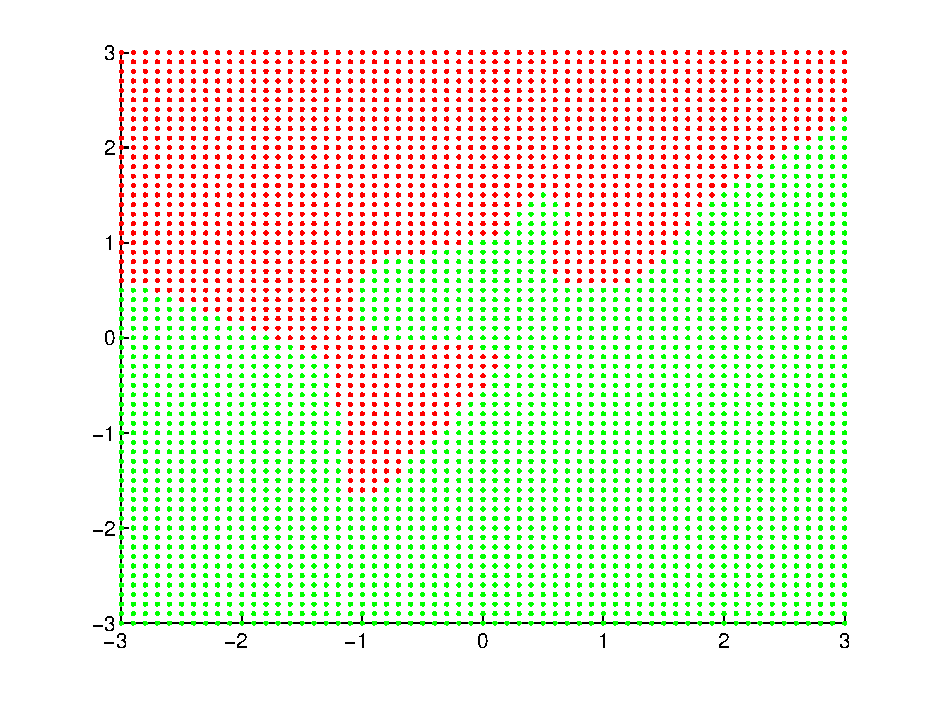
\includegraphics[width=0.6\textwidth]{./images/q23a.pdf}
  \caption{The original prediction trend, $p(\mathbf{x}|\mathcal{C}_k)$}
  \label{fig:q23a}
\end{figure}

\begin{figure}[!htbp]
  \centering
  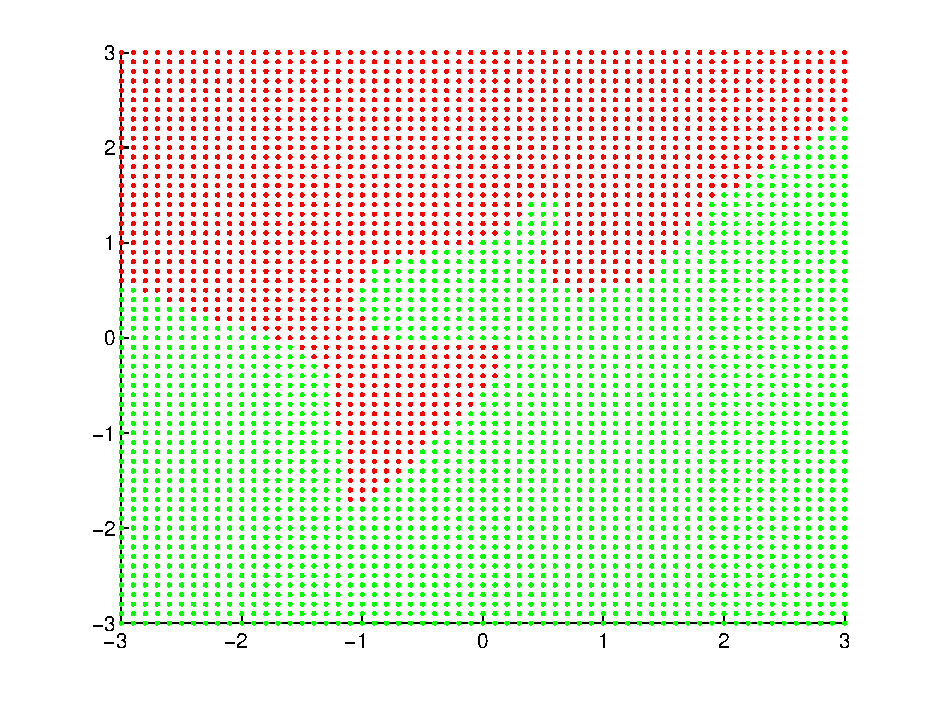
\includegraphics[width=0.6\textwidth]{./images/q23b.pdf}
  \caption{The prediction trend of the Bayes classifikation, $p(\mathbf{x}|\mathcal{C}_k)$}
  \label{fig:q23b}
\end{figure}

As it can be seen, in figure \ref{fig:q23c}, chancing the prior of one of
the classes. Makes it more or less dominent.

\begin{figure}[!htbp]
  \centering
  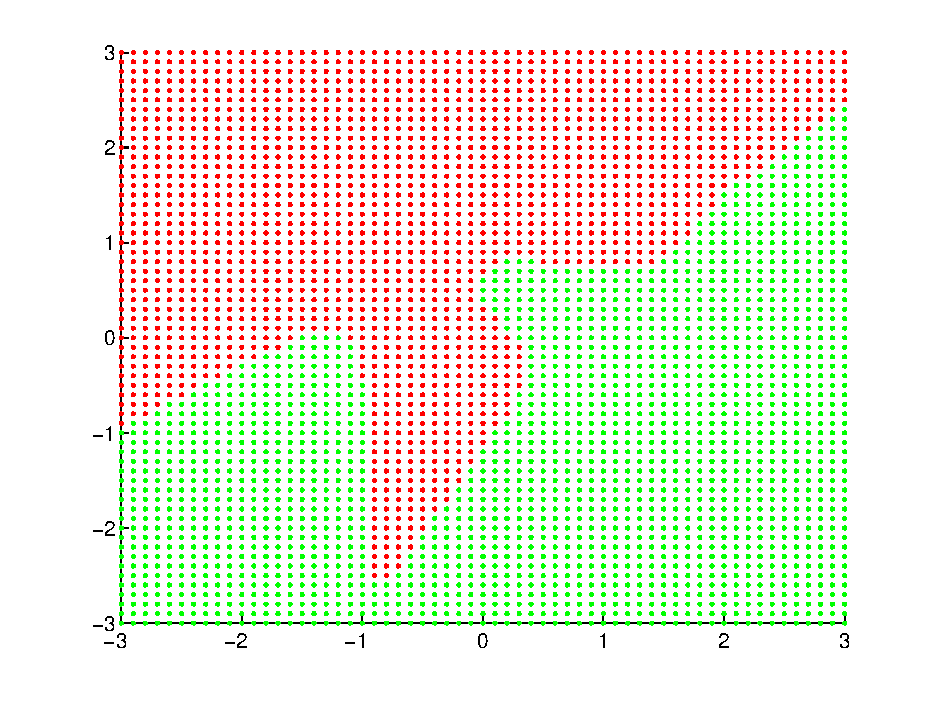
\includegraphics[width=0.6\textwidth]{./images/q23c.pdf}
  \caption{The prediktion trend of the Bayes classification, where class one, have a prior of 1.5}
  \label{fig:q23c}
\end{figure}


\subsection*{Question 2.6}

Setting the two equations equal as follows
\begin{align*}
p(x_1|\mathcal{C}_k)p(x_2|\mathcal{C}_k)p(\mathcal{C}_k) & = \frac{p(\mathcal{C}_k | x_1)p(\mathcal{C}_k | x_2)}{p(\mathcal{C}_k)} \iff \\
p(x_1|\mathcal{C}_k)p(x_2|\mathcal{C}_k)p(\mathcal{C}_k)p(\mathcal{C}_k) & = p(\mathcal{C}_k | x_1)p(\mathcal{C}_k | x_2) \iff
\end{align*}

Using Bayes theorem, we can rewrite
\[
p(\mathcal{C}_k | x_i) = \frac{p(x_i | \mathcal{C}_k)p(\mathcal{C}_k)}{p(x_i)}
\]
We do this for both factors on the right hand side and obtain

\begin{align*}
p(x_1|\mathcal{C}_k)p(x_2|\mathcal{C}_k)p(\mathcal{C}_k)p(\mathcal{C}_k) & = p(\mathcal{C}_k | x_1)p(\mathcal{C}_k | x_2) \iff \\
p(x_1|\mathcal{C}_k)p(x_2|\mathcal{C}_k)p(\mathcal{C}_k)p(\mathcal{C}_k) & = \frac{p(x_1|\mathcal{C}_k)p(\mathcal{C}_k)p(x_2|\mathcal{C}_k)p(\mathcal{C}_k)p(\mathcal{C}_k)}{p(x_1)p(x_2)} \iff \\
\frac{p(x_1|\mathcal{C}_k)p(x_2|\mathcal{C}_k)p(\mathcal{C}_k)p(\mathcal{C}_k)}{p(x_1|\mathcal{C}_k)p(\mathcal{C}_k)p(x_2|\mathcal{C}_k)p(\mathcal{C}_k)} & = p(x_1)p(x_2)
\end{align*}

We therefore see that the normalization constant is $p(x_1)p(x_2)$.

This can also be seen by applying Bayes theorem to $p(\mathcal{C}_k|x_1, x_2)$
\begin{equation*}
p(\mathcal{C}_k|x_1, x_2) = \frac{p(x_1|\mathcal{C}_k)p(x_2|\mathcal{C}_k)p(\mathcal{C}_k)}{p(x_1)p(x_2)}
\end{equation*}
From the above it can be seen that the normalization constant making
sure that the posterior distribution integrates to one is also
$p(x_1)p(x_2)$. As noted in the book the marginal distribution
$p(x_1,x_2)$ do typically not factorize under this model.

The result of running \emph{case26.m} looking at the shared covariance
the contours are simply mirrored in the decision boundary, which is
linear. The independent covariance becomes apperent as the contours of
the densities are formed according to the data the are based
on. Therefore the blue contours are streched more than the red
contours. The decision boundary resembles a hyperbola as in question
2.4.


\subsection*{Question 2.7}

Figure \ref{fig:q27.1} shows the error as a function of $k$.  The
error seems to be lowest when $k = 7$. When $k < 7$ the decisions are
made from too few points, and over-fitting will occur.  Larger values
of $k$ will cause the model to be too simple.

\begin{figure}[!htbp]
  \centering
  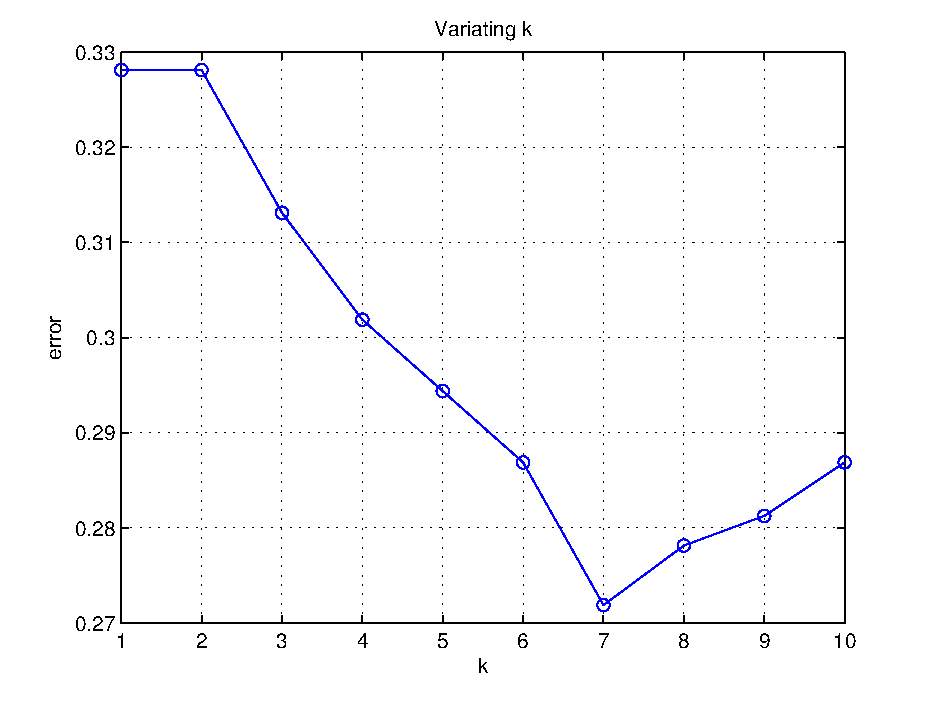
\includegraphics[width=0.6\textwidth]{./images/q207_best_k.pdf}
  \caption{Test error for variating N with 200 training points.}
  \label{fig:q27.1}
\end{figure}

Figure \ref{fig:q27.2} shows the optimal values of $k$ for different
number of points $N$ in the training set.  Seemingly, as $N$ grows,
$k$ needs to be larger for the error to be minimized (apart from the
spike around $50-70$).  This seems reasonable, as the additional
training points will cause the model to be more prone to over-fitting.
When more training points are used, but $k$ is raised correspondingly,
the level of detail, and therefore the error, in the model will remain
optimal.

\begin{figure}[!htbp]
  \centering
  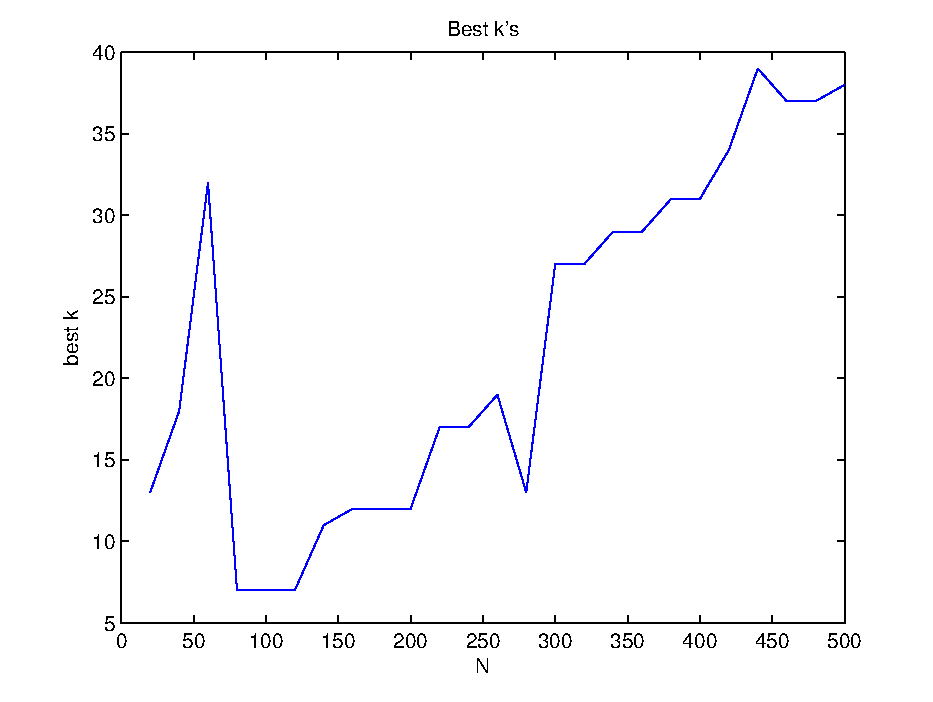
\includegraphics[width=0.6\textwidth]{./images/q207_best_ks.pdf}
  \caption{Best k's (lowest test error) for variating N.}
  \label{fig:q27.2}
\end{figure}


\subsection*{Question 2.8}
\subsubsection*{1)}
Below in figure \ref{fig:q28decisiontree} can be seen the decision
tree for the situation.

% Sets the branch height.
%\branchheight{10em}
\begin{figure}[!htbp]
  \centering
  \synttree[\fbox{{}\quad{}} [No operation, $U(3)$\quad {}][\setlength{\unitlength}{0.5mm} \begin{picture}(1, 1) \put(-1,3){\circle{8}} \end{picture}[Live, $p=\frac{7}{10}$, $U(12)$][Die, $p = \frac{3}{10}$, $U(0)$]]]
  \caption{}
  \label{fig:q28decisiontree}
\end{figure}

\subsubsection*{2)}
The operation should be prefered if $U(3) < 0.7$, this is because in
order to obtain $U(12) = 1.0$, we need to have the operation. And as
there is $p(survive operation) = 0.7$, this results in $1.0 * 0.7 =
0.7$. Whereas the contrary $p(not survive operation) = 1 - p(survive
operation) = 1 - 0.7 = 0.3$, with $U(0) = 0.0$ we get $0.3 * 0.0 =
0.0$

\subsubsection*{3)}
We are to explain the calculations. It is simply a using Bayes theorem
to derive the posterior probability $p(\textrm{survive}|\textrm{pos})$
of the patient surviving given that the test was positive.

\subsubsection*{4)}
Yes, Dr. No should perform the operation, the chances of survival are
as given by the posterior probability in $3)$. Although there are
always a chance that it will fail and the patient will die.


\subsection*{Question 2.9}

The loss matrix describes the cost for each misclassification.
In the given matrix, a misclassification that diagnoses a healthy patient as having cancer costs 1 (just like when no cost matrix is used), but a cancerous patient classified as healthy has a cost of 1000.
In this way, many healthy patients may be misdiagnosed, but few cancerous patients are misdiagnosed; just as one would expect.
The cost of correctly diagnosing a patient, cancerous or not, is of course set to $0$ in the matrix.

Figure \ref{fig:q29} shows the prediction trend when the loss matrix form the assignment is used.
As expected, the cancer predictions now outweigh the healthy predictions by far.
The overall trend is the same as before, i.e. the the healthy predictions are mainly in the lower right corner, but also in the lower left corner.
The border between the predictions are, however, moved away from the cancer predictions, causing an abundance of cancer predictions, just as we would expect.

\begin{figure}[!htbp]
  \centering
  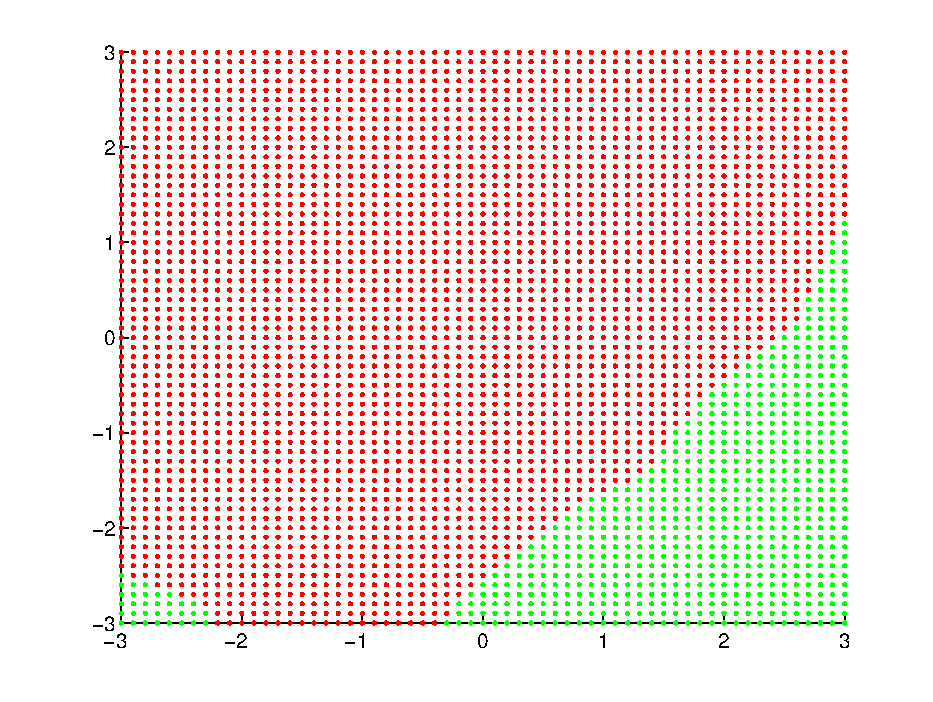
\includegraphics[width=0.6\textwidth]{./images/q209.pdf}
  \caption{The prediction trend when the loss matrix is used. Red dots are cancer predictions; green are healthy.}
  \label{fig:q29}
\end{figure}


\subsection*{Question 2.10}

We are to try out various numbers of hidden units in the neural
network. From figure \ref{fig:q210hidden} we see that using $260$
hidden units performs the best on the test data with $27.31\%$
error. The resulting decision boundaries can be seen in figure
\ref{fig:q210Nh260}. The boundary is rather complex due to the large
number of hidden units within the network. As another example figure
\ref{fig:q210Nh2} shows decision boundaries using only $2$ hidden
units. This results in a nearly linear boundary, due to the
inflexibility of using only $2$ hidden units. As opposed to $2$ and
$260$ hidden units, figure \ref{fig:q210Nh1000} shows the result of
using $1000$ hidden units. We now have a situation where we have low
misclassification rate on the training data scoring $22.00\%$ error,
but the model do not generalize very well resulting in $29.12\%$ on
the test data. From the figure it can be seen that the model tends
towards overfitting, by having more curvatures.

\begin{figure}[!htbp]
  \centering
  \subfloat[\label{subfig:q210Nh10}]{
  \begin{tabular}{|c|c|}
    \hline
    \multicolumn{2}{|c|}{Hidden units $= 10$} \\
    \hline
    Training error: 24.67\% & Test error: 29.38\% \\
    \hline
  \end{tabular}
  }
  \subfloat[\label{subfig:q210Nh30}]{
    \begin{tabular}{|c|c|}
      \hline
      \multicolumn{2}{|c|}{Hidden units $= 30$} \\
      \hline
      Training error: 25.33\% & Test error: 28.75\% \\
      \hline
    \end{tabular}
  } \\
  \subfloat[\label{subfig:q210Nh60}]{
    \begin{tabular}{|c|c|}
      \hline
      \multicolumn{2}{|c|}{Hidden units $= 60$} \\
      \hline
      Training error: 23.33\% & Test error: 28.00\% \\
      \hline
    \end{tabular}
  } 
  \subfloat[\label{subfig:q210Nh100}]{
    \begin{tabular}{|c|c|}
      \hline
      \multicolumn{2}{|c|}{Hidden units $= 100$} \\
      \hline
      Training error: 22.67\% & Test error: 28.31\% \\
      \hline
    \end{tabular}
  } \\
  \subfloat[\label{subfig:q210Nh130}]{
    \begin{tabular}{|c|c|}
      \hline
      \multicolumn{2}{|c|}{Hidden units $= 130$} \\
      \hline
      Training error: 22.67\% & Test error: 28.12\% \\
      \hline
    \end{tabular}
  } 
  \subfloat[\label{subfig:q210Nh200}]{
    \begin{tabular}{|c|c|}
      \hline
      \multicolumn{2}{|c|}{Hidden units $= 200$} \\
      \hline
      Training error: 23.33\% & Test error: 27.88\% \\
      \hline
    \end{tabular}
  } \\
  \subfloat[\label{subfig:q210Nh260}]{
    \begin{tabular}{|c|c|}
      \hline
      \multicolumn{2}{|c|}{Hidden units $= 260$} \\
      \hline
      Training error: 22.67\% & Test error: \textbf{27.31\%} \\
      \hline
    \end{tabular}
  } 
  \subfloat[\label{subfig:q210Nh300}]{
    \begin{tabular}{|c|c|}
      \hline
      \multicolumn{2}{|c|}{Hidden units $= 300$} \\
      \hline
      Training error: 24.00\% & Test error: 27.81\% \\
      \hline
    \end{tabular}
  } \\
  \subfloat[\label{subfig:q210Nh500}]{
    \begin{tabular}{|c|c|}
      \hline
      \multicolumn{2}{|c|}{Hidden units $= 500$} \\
      \hline
      Training error: 22.67\% & Test error: 29.31\% \\
      \hline
    \end{tabular}
  } 
  \subfloat[\label{subfig:q210Nh1000}]{
    \begin{tabular}{|c|c|}
      \hline
      \multicolumn{2}{|c|}{Hidden units $= 1000$} \\
      \hline
      Training error: \textbf{22.00\%} & Test error: 29.12\% \\
      \hline
    \end{tabular}
  }
  \caption{Show the result of running the neural network with various numbers of hidden units.}
  \label{fig:q210hidden}
\end{figure}

\begin{figure}[!htbp]
  \centering
  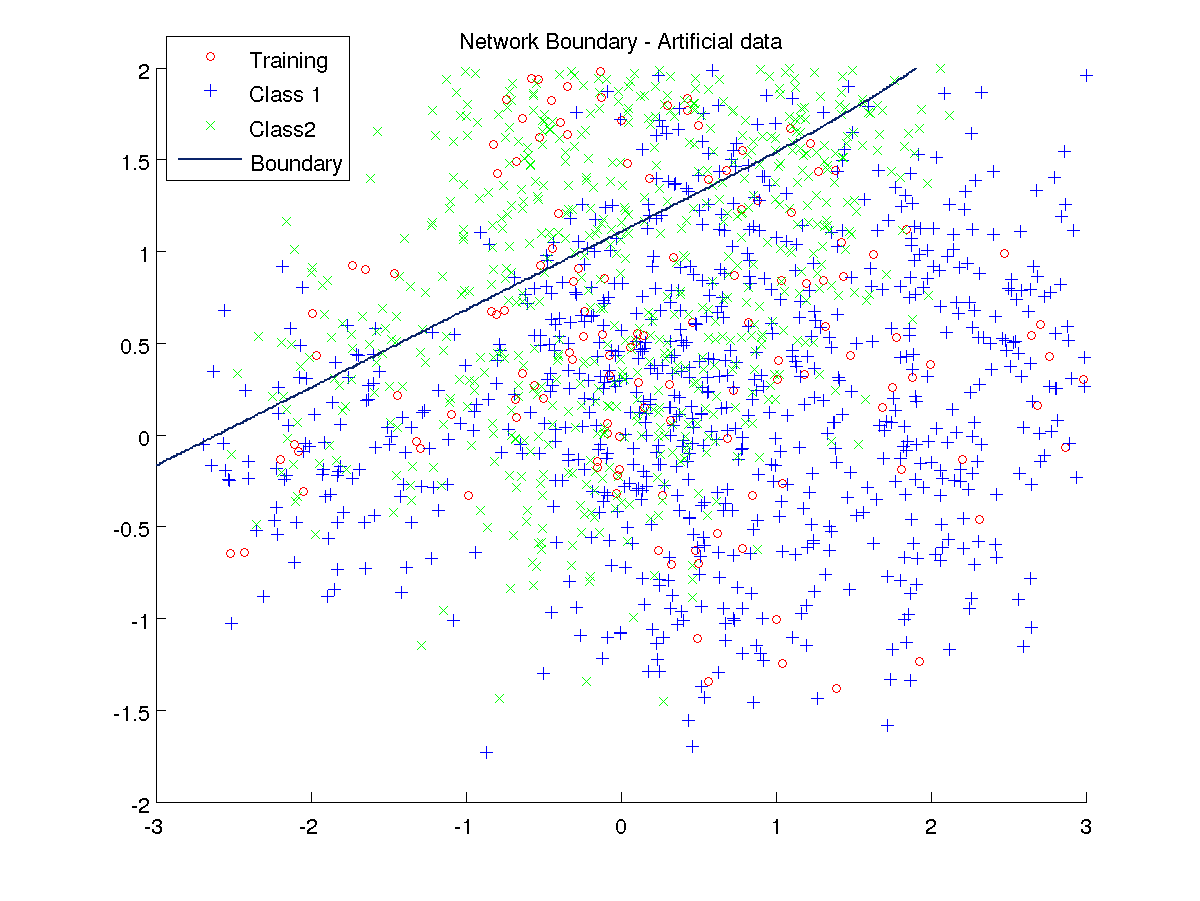
\includegraphics[width=1.0\textwidth]{./images/q210a_Nh2}
  \caption{}
  \label{fig:q210Nh2}
\end{figure}

\begin{figure}[!htbp]
  \centering
  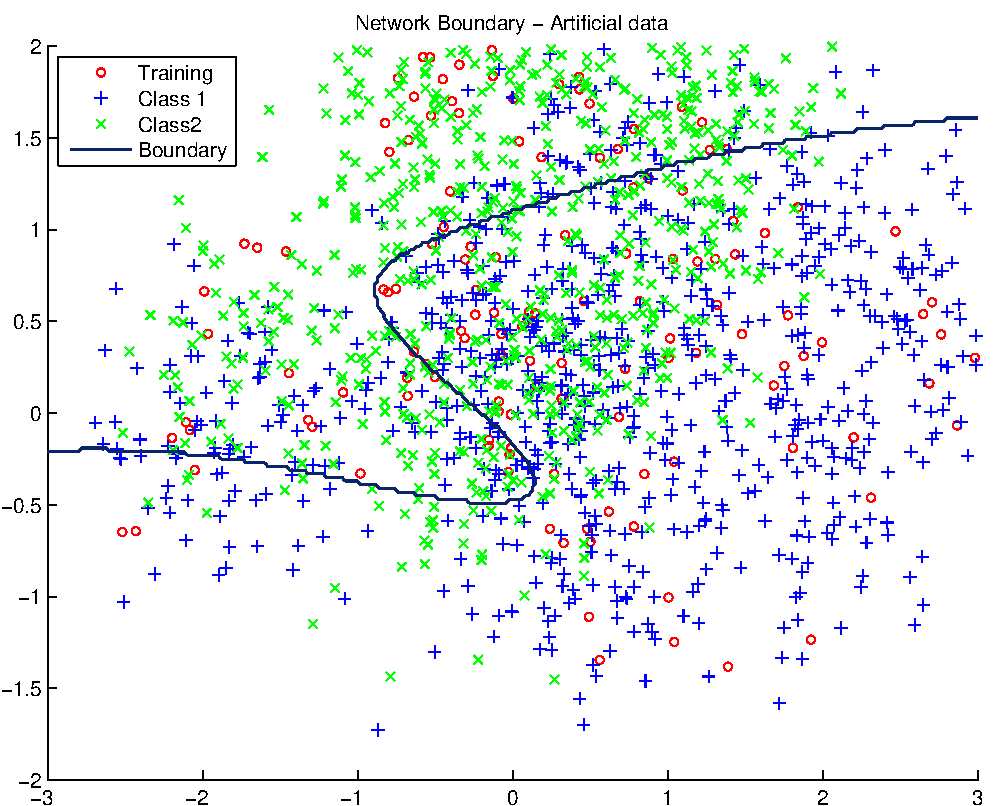
\includegraphics[width=1.0\textwidth]{./images/q210a_Nh260}
  \caption{}
  \label{fig:q210Nh260}
\end{figure}

\begin{figure}[!htbp]
  \centering
  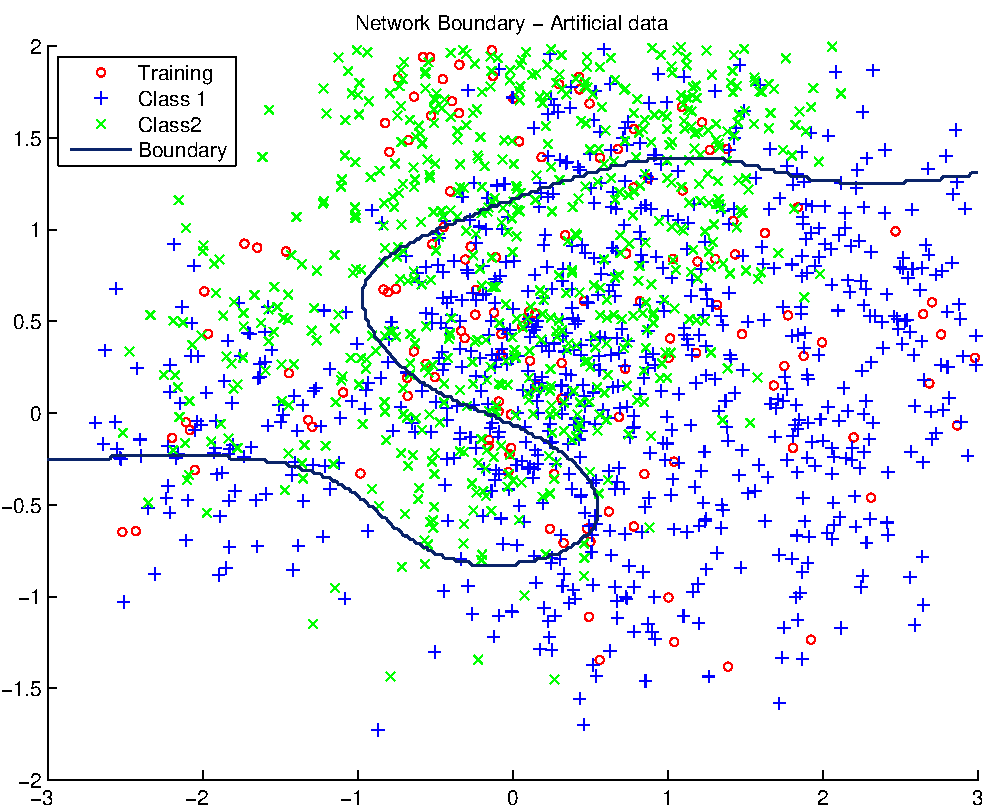
\includegraphics[width=1.0\textwidth]{./images/q210a_Nh1000}
  \caption{}
  \label{fig:q210Nh1000}
\end{figure}

In figure \ref{fig:q1_1} can be seen the $100$ data points drawn from
the gaussian distribution with $\mu = [1.0~ 1.0]$ and $\Sigma = [0.3~
  0.2; 0.2~ 0.2]$. The correct $\mu$ is blue and $\widehat{\mu}$ is
marked with red.

\begin{figure}[!htpb]
  \centering
%  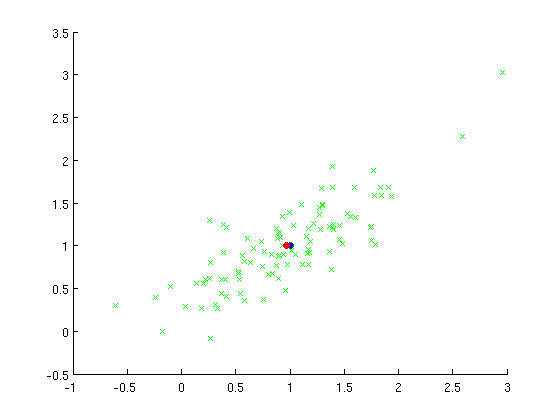
\includegraphics[width=0.6\textwidth]{images/q1_1}
  \caption{100 data points, correct mean with blue and estimated mean red.}
  \label{fig:q1_1}
\end{figure}

To quantify how much the estimated mean deviates from the correct
mean, we use usual euclidean distance between the two vectors.

Our distance is $0.0392$, which is not very much. This can also be
seen from the drawing, the points are placed really close.

The covariance matrix is also calculated on the training data:\\
$$\Sigma _{ML} = \left[
  \begin {array}{ccc}
    0.0082 & 0.0052 & 0.0067\\
    \noalign{\medskip}
    0.0052 & 0.0171 & 0.0199\\
    \noalign{\medskip}
    0.0067 & 0.0199 & 0.0241\\
  \end {array}
  \right]$$
% [0.0082~ 0.0052~ 0.0067; 0.0052~ 0.0171~ 0.0199; 0.0067~ 0.0199~ 0.0241]


\subsection*{Question 2.11}

As seen in figure \ref{fig:q211.1} through \ref{fig:q211.3}, the
penalization parameter controls how much the green points are weighed
compared to the blue ones.

\begin{figure}[!htbp]
  \centering
  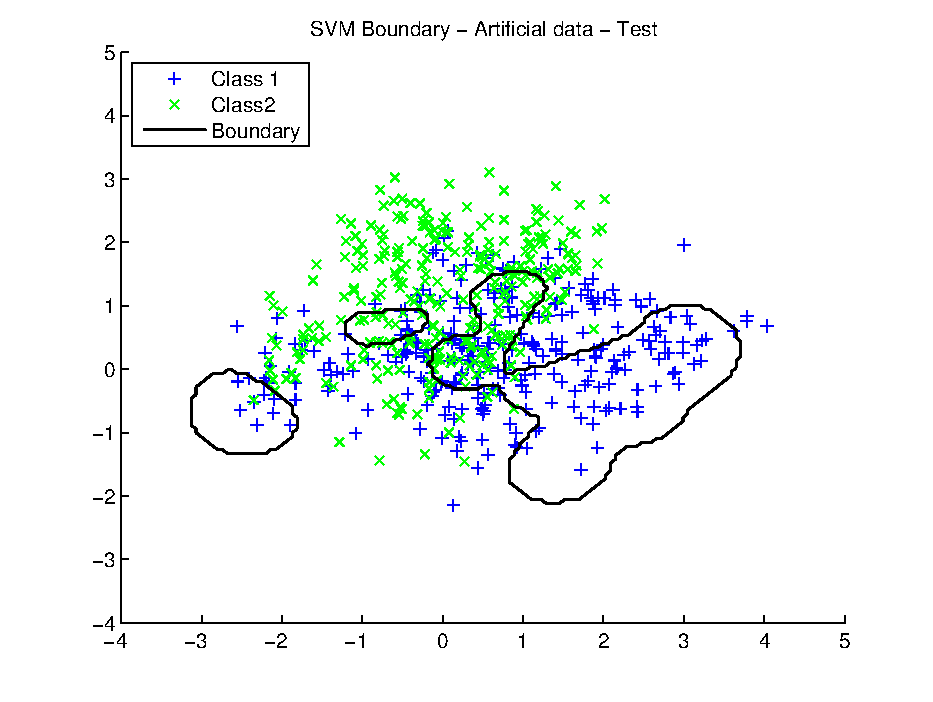
\includegraphics[width=0.6\textwidth]{./images/q211_0_1.pdf}
  \caption{Boundary when the penalization parameter is set to $0.1$.}
  \label{fig:q211.1}
\end{figure}
\begin{figure}[!htbp]
  \centering
  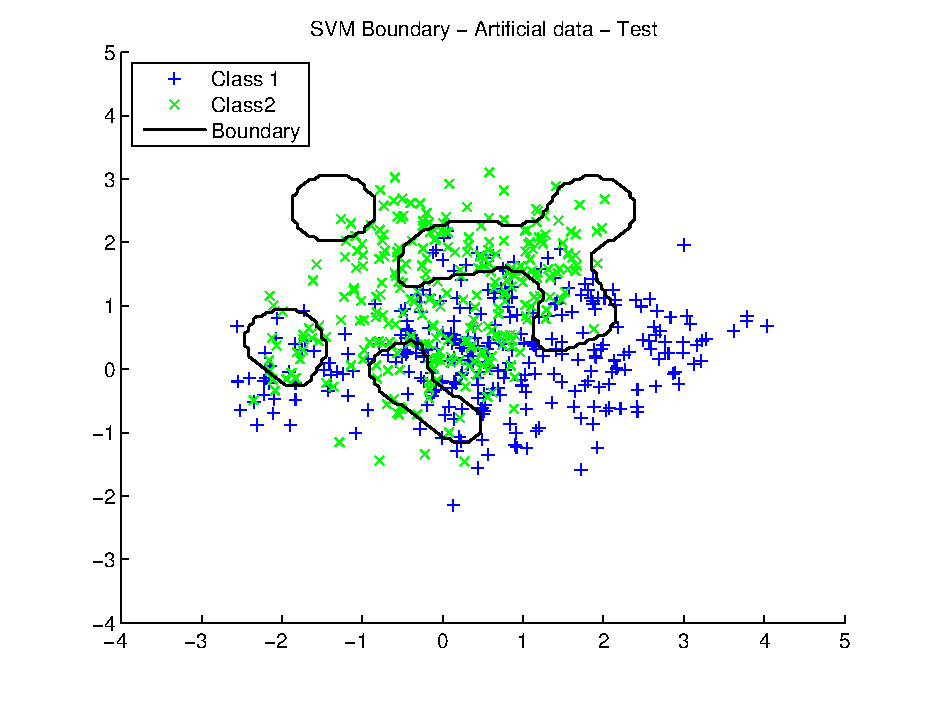
\includegraphics[width=0.6\textwidth]{./images/q211_01.pdf}
  \caption{Boundary when the penalization parameter is set to $1$.}
  \label{fig:q211.2}
\end{figure}
\begin{figure}[!htbp]
  \centering
  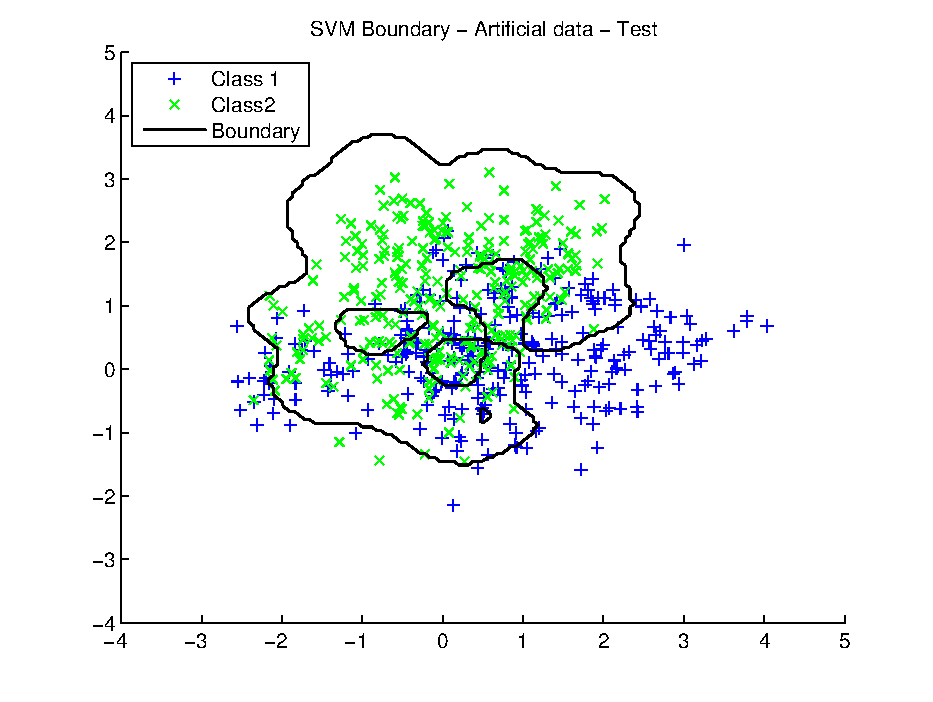
\includegraphics[width=0.6\textwidth]{./images/q211_10.pdf}
  \caption{Boundary when the penalization parameter is set to $10$.}
  \label{fig:q211.3}
\end{figure}

The general trend of the error as a function of the penalization
parameter can be seen in figure \ref{fig:q211.4}.  When variating the
length scale of the kernel function, the error variates as seen in
figure \ref{fig:q211.5}.

\begin{figure}[!htbp]
  \centering
  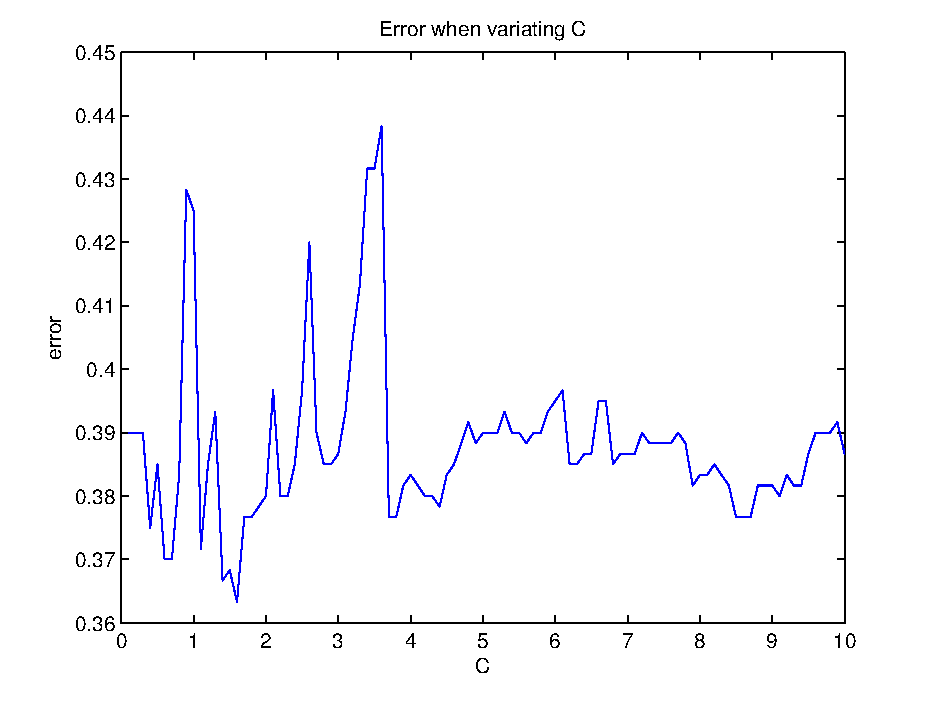
\includegraphics[width=0.6\textwidth]{./images/q211_errors.pdf}
  \caption{Error when variating the penalization parameter.}
  \label{fig:q211.4}
\end{figure}
\begin{figure}[!htbp]
  \centering
  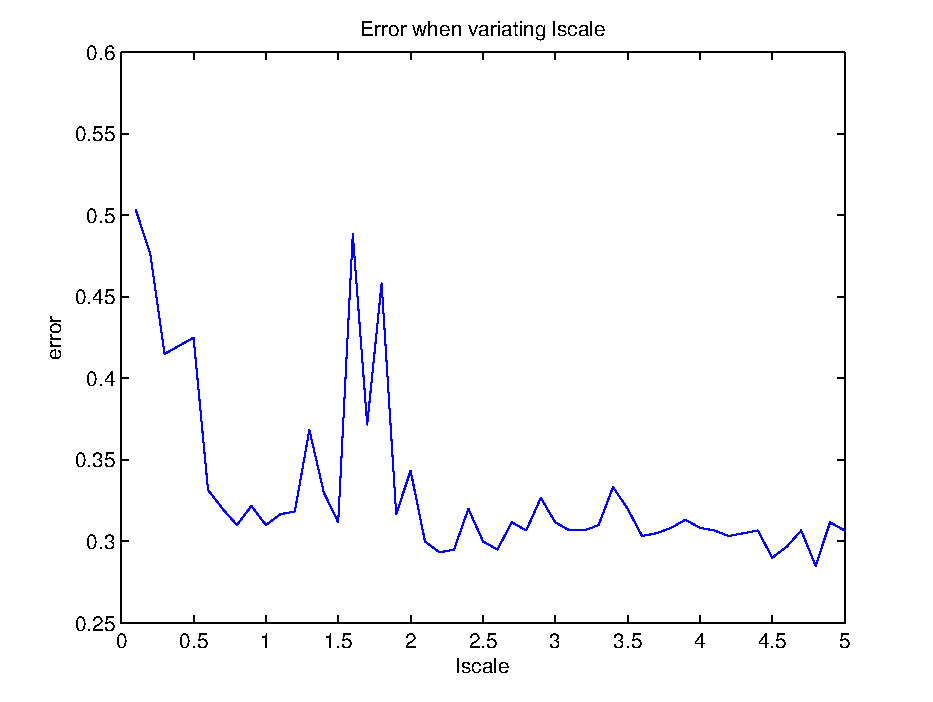
\includegraphics[width=0.6\textwidth]{./images/q211_errors_lscale.pdf}
  \caption{Error when variating the length scale of the kernel function.}
  \label{fig:q211.5}
\end{figure}



%%%%%%%%%%%%%%%%%%%%%%%%%%%%%%%%%%%%%%%%%%%%%%%%%%%%%%%%%%%%%%%%%%%%
% Formal stuff

%\bibliographystyle{abbrvnat}
%\bibliography{bibliography}
%\addcontentsline{toc}{chapter}{Litteratur

\end{document}
